%%%%%%%%%%%%%%%%%%%%%%%%%%%%%%%%%%%%%%%%%%%%%%%%%%%%%%%%%%%%%%%%%%%%%%%%%%%%
\documentclass[a4j]{jarticle}

\usepackage{jsaisig}
\usepackage[dvipdfmx]{graphicx}

%%%%%%%%%%%%%%%%%%%%%%%%%%%%%%%%%%%%%%%%%%%%%%%%%%%%%%%%%%%%%%%%%%%%%%%%%%%

\begin{document}

% 和文タイトル
\title{ソフトウェア工学}

\author{E1237 森 篤史}


\maketitle
\thispagestyle{empty}

%%%%%%%%%%%%%%%%%%%%%%%%%%%%%%%%%%%%%%

\section{文章化}
\begin{itemize}
 \item このプログラムはある大きさのイラストロジックの答えを割り出すプログラムである。
 \item イラストロジックを解き、その解を画面に出力する。
 \item イラストロジックには解を書き込む解エリアと、ヒントを与える出題エリアがある。
 \item 解エリアは長方形をしていて、$n\times m$個の回答マスによって構成されている。
 \item 解エリアのそれぞれの出題マスには、塗るマス(黒マス)か塗らないマス(白マス)かの2値が入力さ左部に$y \times m$のマスによって構成されている。
 \item 上部の出題エリアはそれぞれその列の、左部の出題エリアにはそれぞれその行に塗るマスのヒントとなる数字が書かれている。
 \item 1個の数字は連続する黒マスの数を表している。
 \item 数字が複数ある場合、それぞれが連続で黒マスの数を表し、間には必ず白マスが最低1つ入る。
\end{itemize}

\section{名刺の抽出}
\subsection{仕様書から抽出された名刺}
イラストロジック、画面、解エリア、長方形、回答マス、出題マス、出題エリア、黒マス、白マス、数字、列、行

\subsection{クラス候補}
イラストロジック、解エリア、出題エリア、数字、回答マス、出題マス、列、行

\section{関連の洗い出し}
図\ref{fig:class-relation}に関連を反映したクラス図を示す。

\begin{figure}[hp]
\centering
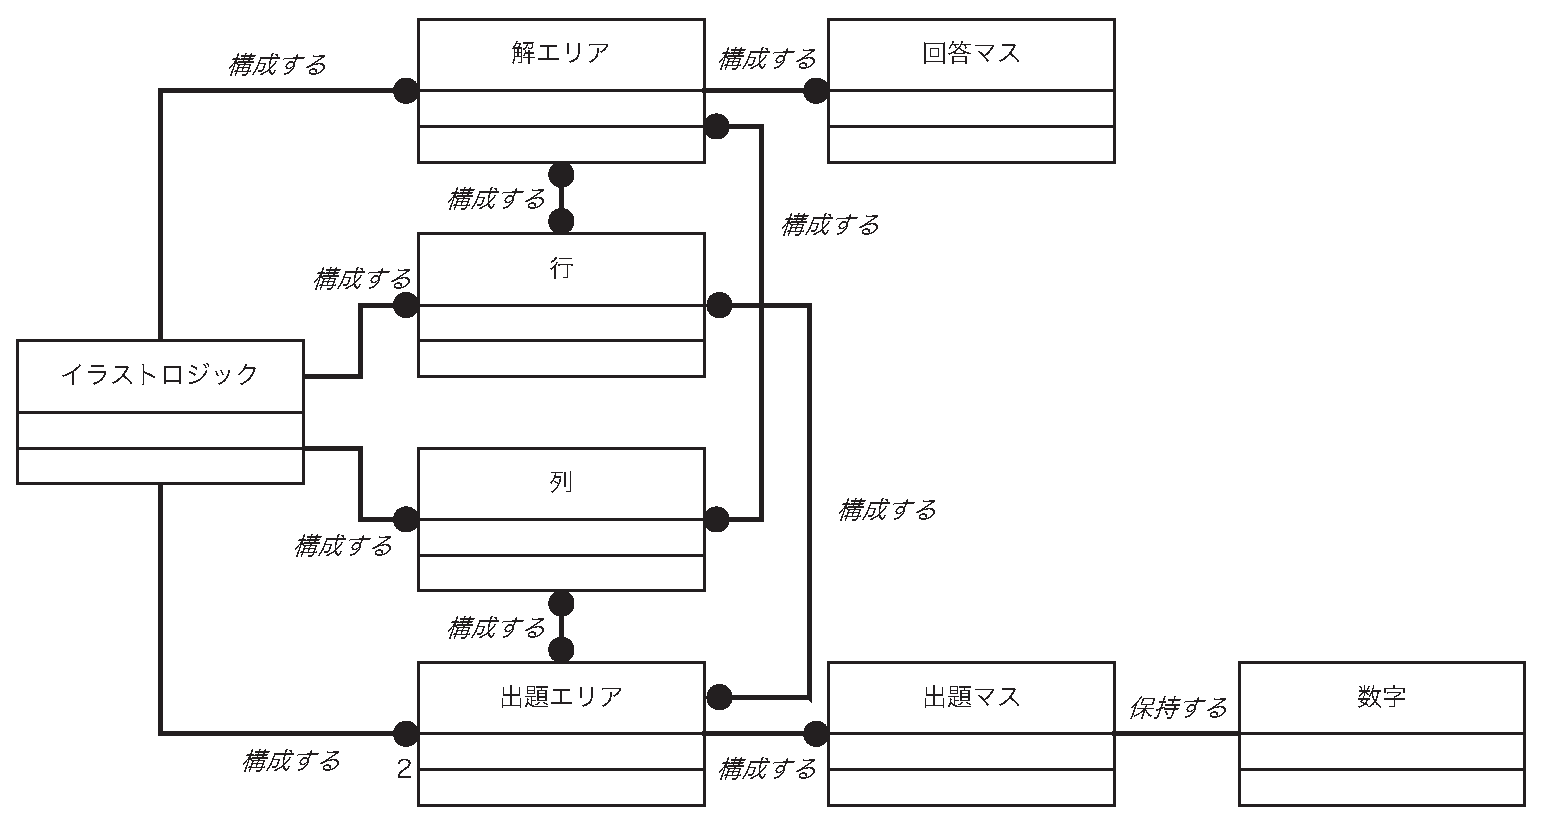
\includegraphics[width=15cm]{./image/class-relation.eps}
\caption{関連を反映させたクラス図}
\label{fig:class-relation}
\end{figure}

\section{操作の洗い出し}
図\ref{fig:class-method}に簡単な操作を書き込んだクラス図を示す。

\begin{figure}[hp]
\centering
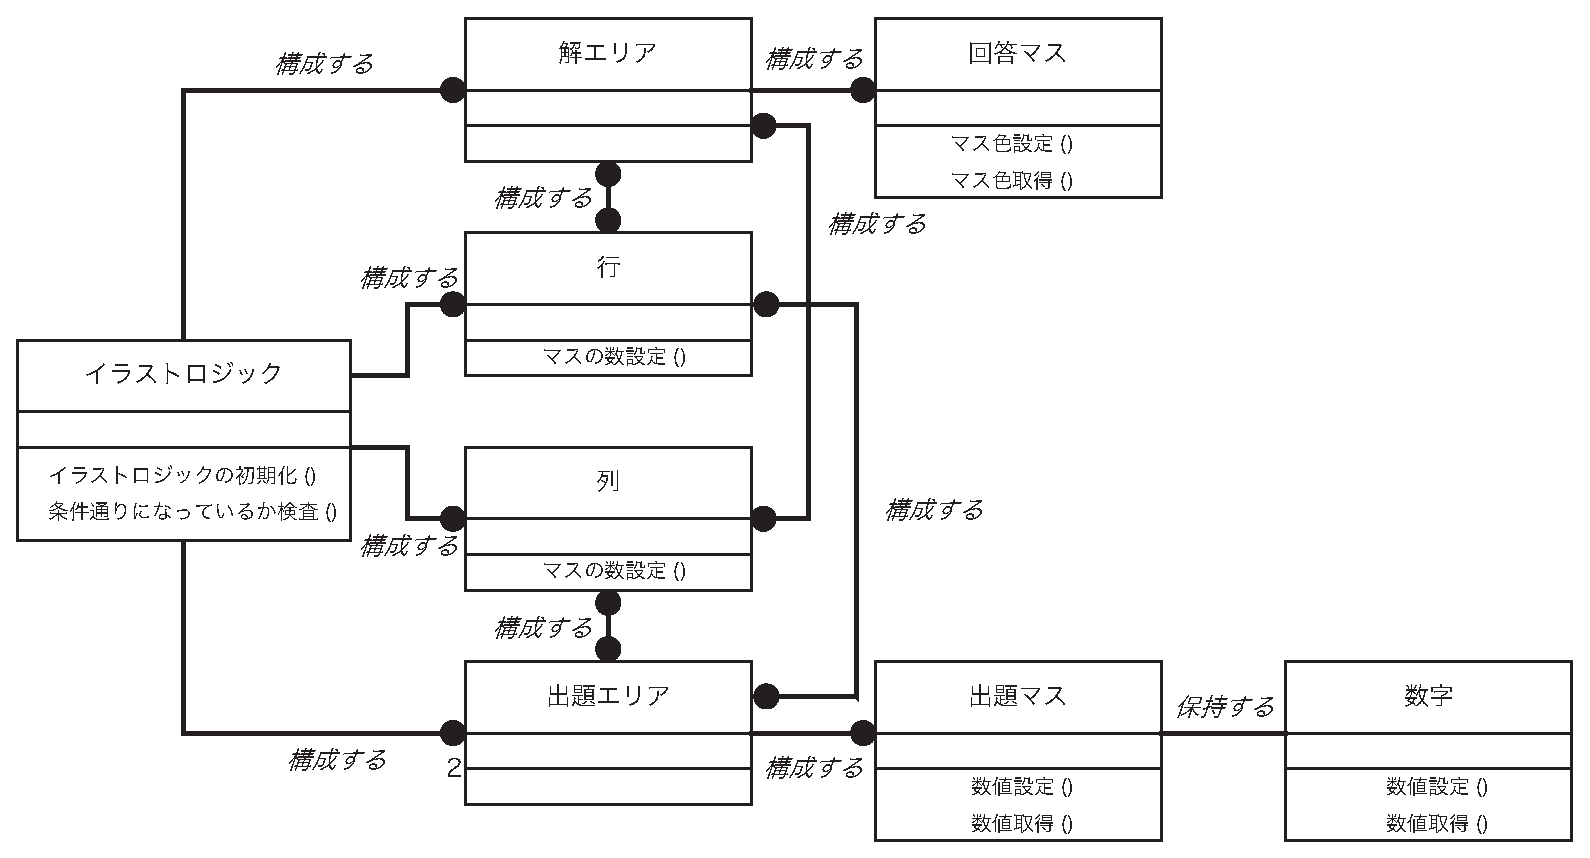
\includegraphics[width=15cm]{./image/class-method.eps}
\caption{簡単な操作を書き込んだクラス図}
\label{fig:class-method}
\end{figure}

\section{属性の洗い出し}
図\ref{fig:class-attribute}に属性を書き込んだクラス図を示す。

\begin{figure}[hp]
\centering
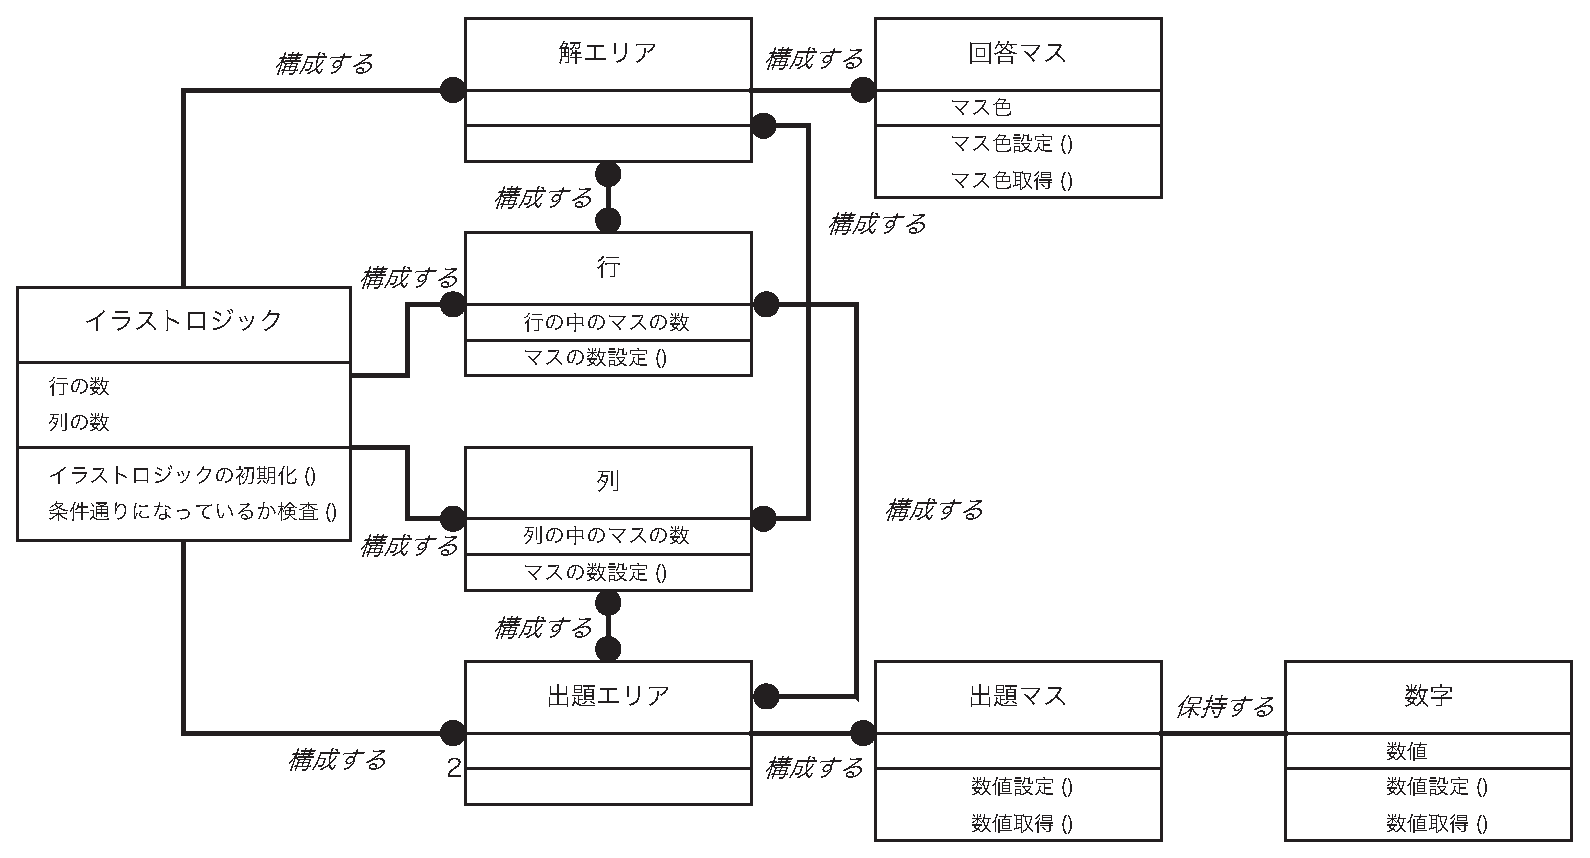
\includegraphics[width=15cm]{./image/class-attribute.eps}
\caption{属性を書き込んだクラス図}
\label{fig:class-attribute}
\end{figure}

\section{動的分析}
\subsection{状態遷移図}
図\ref{fig:state-transition}にアプリケーション全体の状態遷移図を示す。

\begin{figure}[hp]
\centering
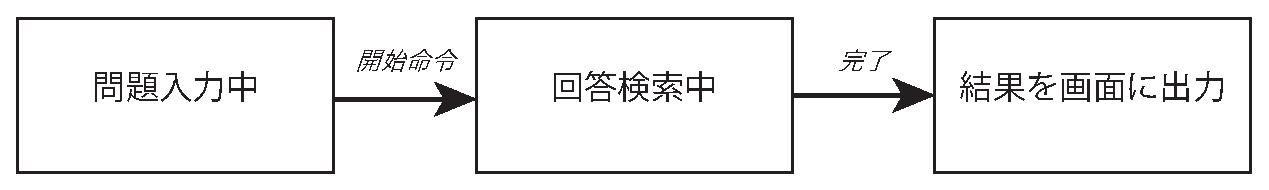
\includegraphics[width=15cm]{./image/state-transition.eps}
\caption{属性を書き込んだクラス図}
\label{fig:state-transition}
\end{figure}

\subsection{シーケンス図}
全体の流れとしては以下のようになる。
\begin{enumerate}
 \item 問題を入力する。
 \item 左部出題エリアより1行取得する。\label{enum:2}
 \item それをもとに、解エリアのその行で答えが確定するマスに回答を書き込む。\label{enum:3}
 \item \ref{enum:2}〜\ref{enum:3}を全行で繰り返す。
 \item 上部出題エリアより1列取得する。\label{enum:5}
 \item それをもとに、解エリアのその列で答えが確定するマスに回答を書き込む。\label{enum:6}
 \item \ref{enum:5}〜\ref{enum:6}を全列で繰り返す。
 \item 全てのマスが確定しているか確認する。確定していれば終了。していなければ\ref{enum:2}に戻る。
\end{enumerate}

図\ref{fig:sequence-diagram}に回答検索のシーケンス図を示す。

\begin{figure}[hp]
\centering
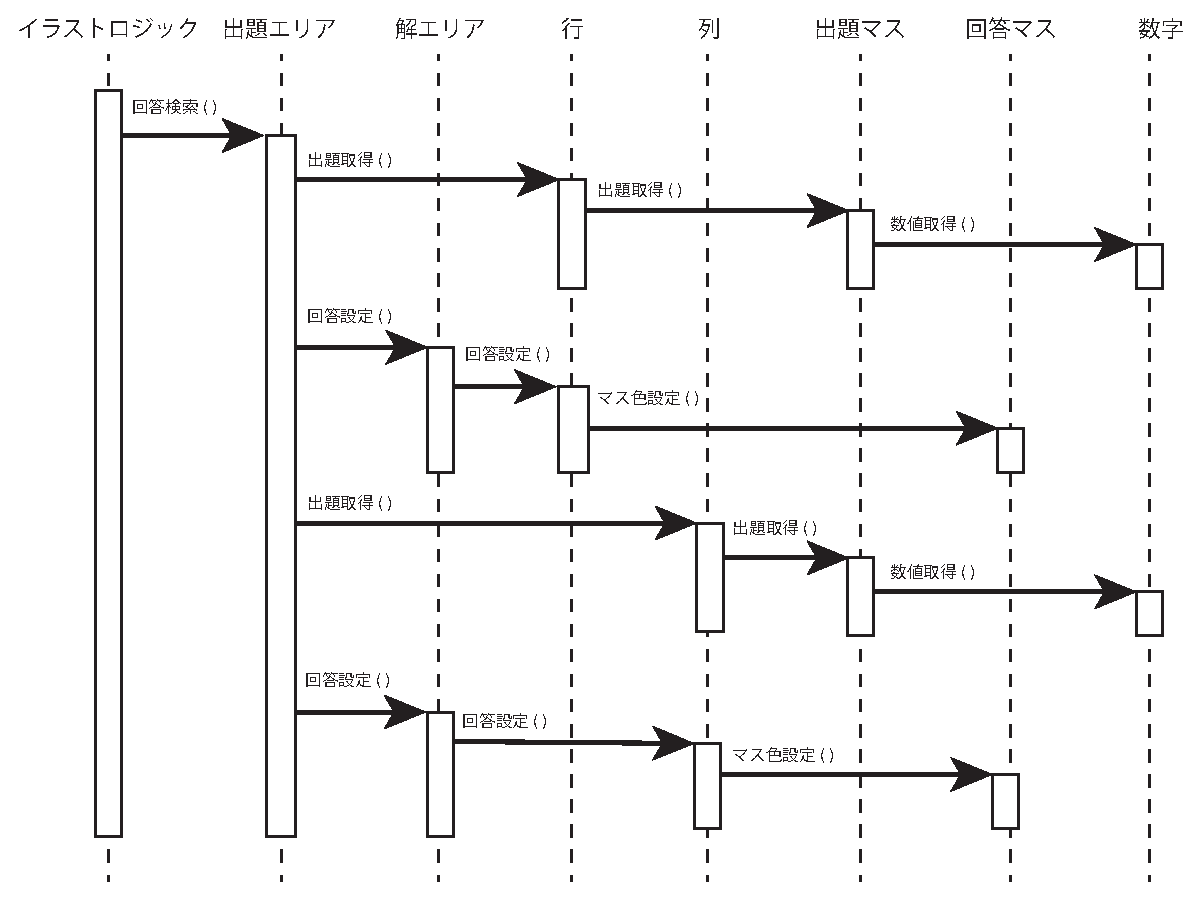
\includegraphics[width=15cm]{./image/sequence-diagram.eps}
\caption{回答検索のシーケンス図}
\label{fig:sequence-diagram}
\end{figure}

\subsection{クラス図の変更}
図\ref{fig:sequence-diagram}のシーケンス図に合わせたクラス図を\ref{fig:class-sequence}に示す。

\begin{figure}[hp]
\centering
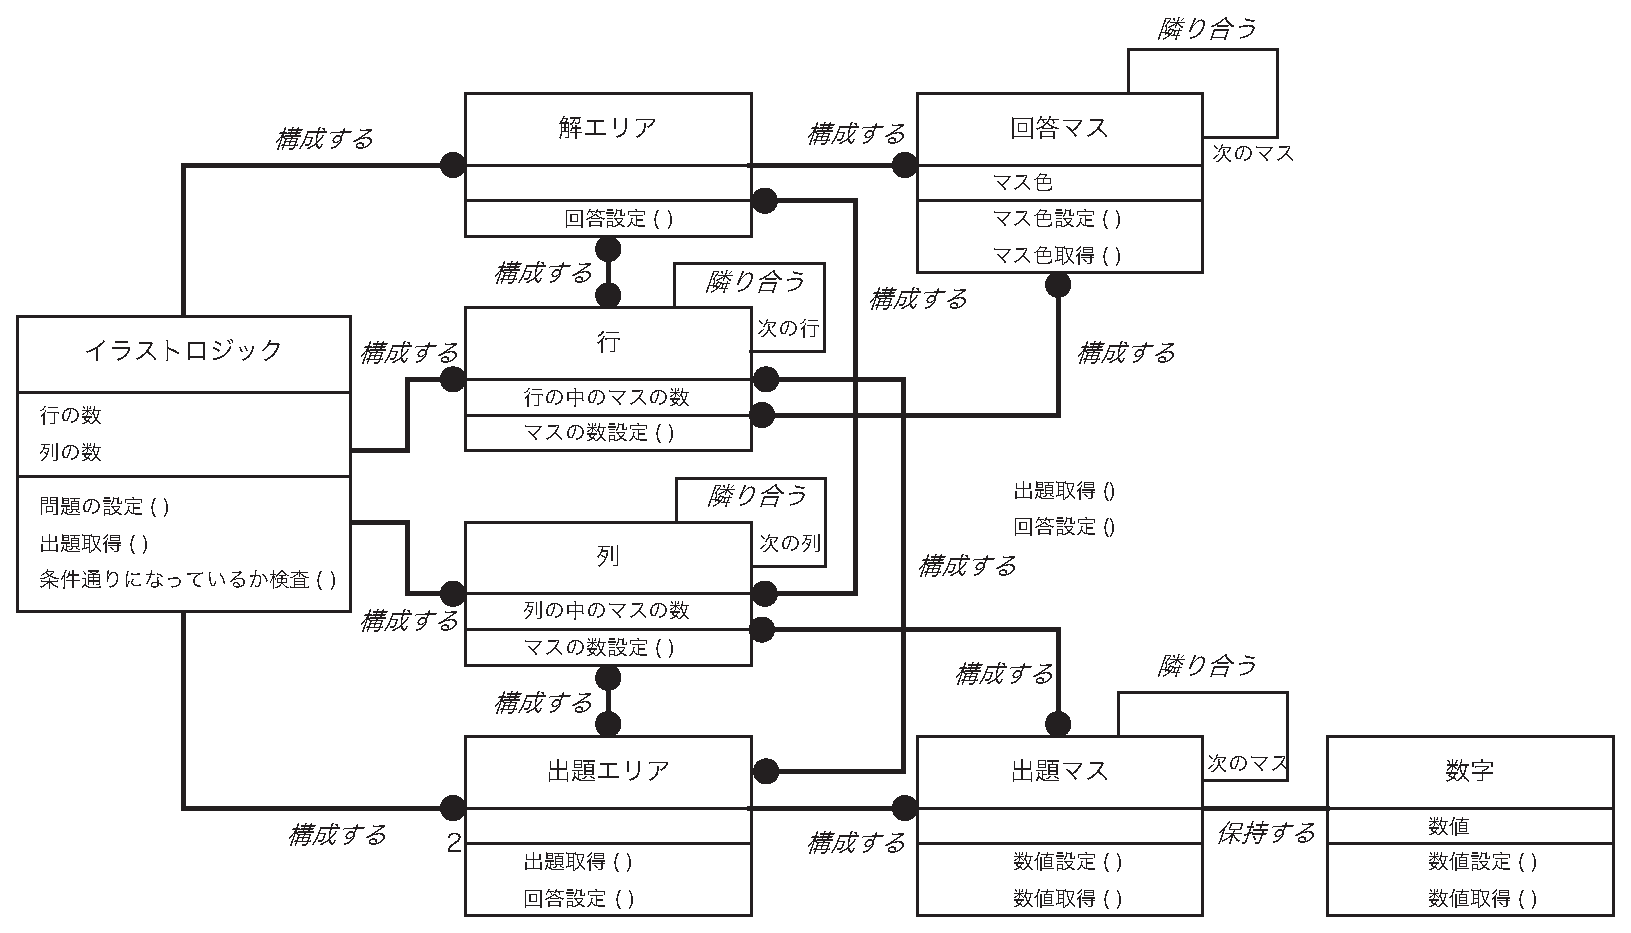
\includegraphics[width=15cm]{./image/class-sequence.eps}
\caption{属性を書き込んだクラス図}
\label{fig:class-sequence}
\end{figure}

\section{クラス図の洗礼}
図\ref{fig:class-absorption}にクラスの吸収を行ったクラス図を示す。

\begin{figure}[hp]
\centering
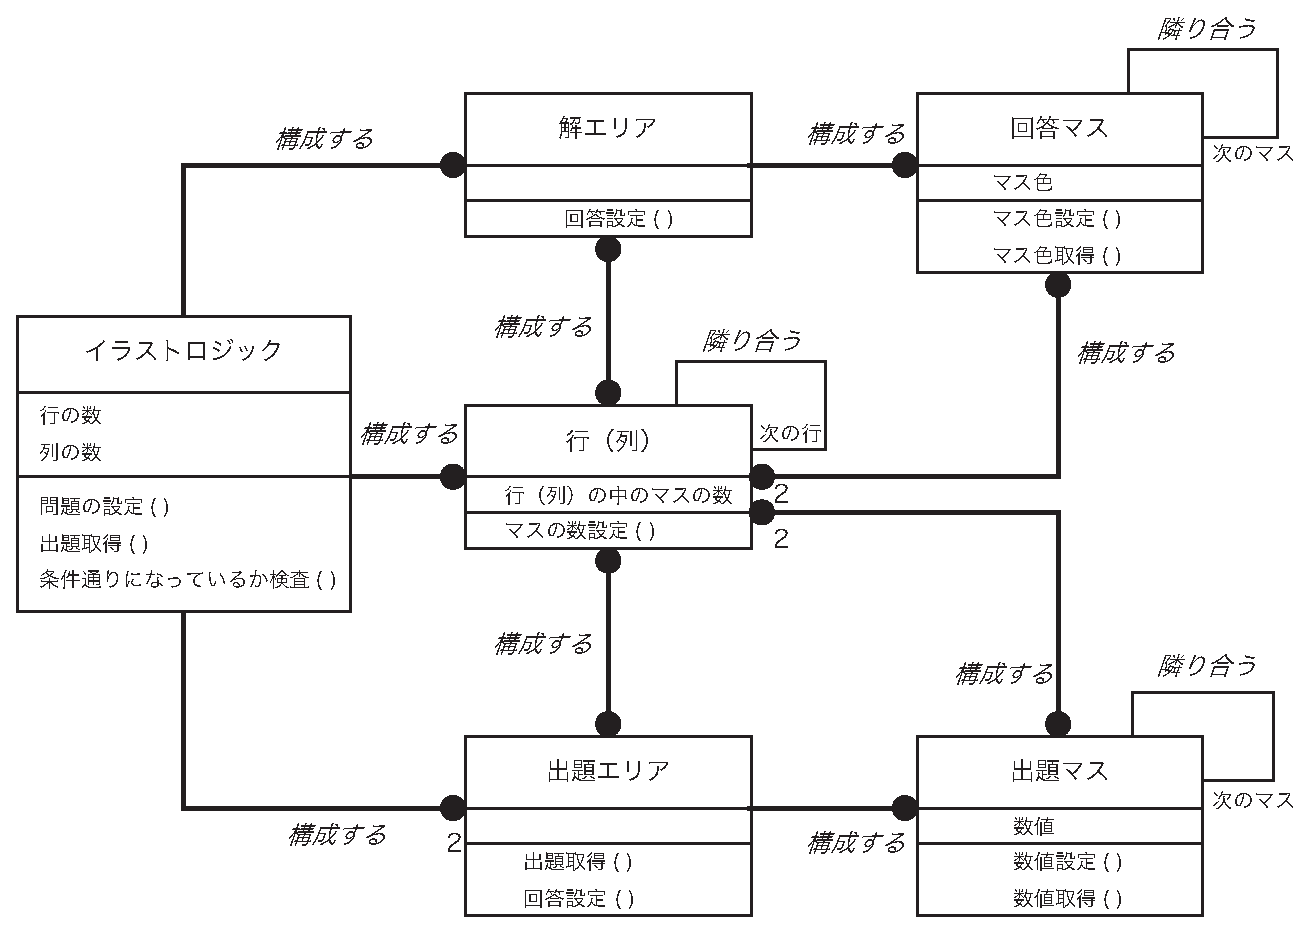
\includegraphics[width=15cm]{./image/class-absorption.eps}
\caption{クラスの吸収を行ったクラス図}
\label{fig:class-absorption}
\end{figure}

\section{アルゴリズム}
出題取得を行った後、回答設定を行うまでのアルゴリズムを以下に記述する。
また、解エリアには黒マス、白マスの他に未確定マスがあるとする。

\begin{enumerate}
 \item 解エリアから一行(一列)を取りし、出題エリアからも同じ行(列)を取り出す。
 \item 出題エリアの行の和が0の場合、全て白マスとし、終了する。
 \item 解エリアの行の中から、白マスを除いたマス数を数える。それが出題エリアの行の和と同じ、もしくは1少なければその行の答えを確定し、終了する。
 \item 解エリアの最初から最初の白マスまでの長さを調べる。その長さが出題エリアの最初の値と同じであれば、そこまで全て黒マスにする。またさらに次の白マスまでの長さを調べ、それが出題エリアの次の値と同じであればさらに黒マスにする。これを繰り返す。
 \item 解エリアの最後から最後の白マスまでの長さを調べる。その長さが出題エリアの最後の値と同じであれば、そこまで全て黒マスにする。またさらに次の白マスまでの長さを調べ、それが出題エリアの次の値と同じであればさらに黒マスにする。これを繰り返す。
 \item 未確定の出題マスが一つになった場合、最初から塗っても、最後から塗っても重なる部分が存在するため、そこを黒マスで確定させる。
\end{enumerate}
以上の作業を行で全てやった後、列で全てやり、また行に戻って繰り返す。

\end{document}

